\documentclass[12pt]{article}
\usepackage{amsmath, amssymb, geometry}
\usepackage{graphicx}
\usepackage{booktabs}
\geometry{margin=1in}
\setlength{\parindent}{0pt}
\setlength{\parskip}{0.6em}

% ---------- Figure placeholder macro ----------
\newcommand{\figplaceholder}[2]{%
\begin{figure}[h!]
\centering
\fbox{%
\begin{minipage}[c][2.1in][c]{0.90\linewidth}
\centering
\textbf{Figure Placeholder: #1}\\[0.4em]
#2
\end{minipage}}
\caption{#1}
\end{figure}
}

\title{Solutions -- Practice Problem Set 3}
\author{ECON 300 -- Labour Economics}
\date{Winter 2026}

\begin{document}
\maketitle


\section*{1. Competitive Labour Market}

Given:
\[
N^S = 20W,\qquad N^D = 400 - 10W.
\]

\subsection*{(a) Competitive equilibrium $(W^*,N^*)$}
Set supply equal to demand:
\[
20W = 400 - 10W
\Rightarrow 30W = 400
\Rightarrow W^* = \frac{400}{30}=\frac{40}{3}\approx 13.33.
\]
Then:
\[
N^* = 20W^* = 20\cdot\frac{40}{3}=\frac{800}{3}\approx 266.67.
\]

\subsection*{(b) Worker surplus and firm surplus (use triangles)}
First write inverse supply and inverse demand.

Supply: $N=20W \Rightarrow W_S(N)=\dfrac{N}{20}$ (passes through the origin).

Demand: $N=400-10W \Rightarrow W_D(N)=40-\dfrac{N}{10}$ (vertical intercept 40).

\textbf{Worker surplus (WS).} Since supply intercept is 0, WS is a triangle with:
\[
\text{height} = W^*,\qquad \text{base} = N^*.
\]
So:
\[
WS = \frac{1}{2}(W^*)(N^*)
= \frac12\left(\frac{40}{3}\right)\left(\frac{800}{3}\right)
= \frac{16000}{9}\approx 1777.78.
\]

\textbf{Firm surplus (FS).} FS is a triangle with:
\[
\text{height}=40-W^*,\qquad \text{base}=N^*.
\]
So:
\[
FS = \frac{1}{2}(40-W^*)N^*
= \frac12\left(40-\frac{40}{3}\right)\left(\frac{800}{3}\right)
= \frac12\left(\frac{80}{3}\right)\left(\frac{800}{3}\right)
= \frac{32000}{9}\approx 3555.56.
\]

\subsection*{(c) Graph}
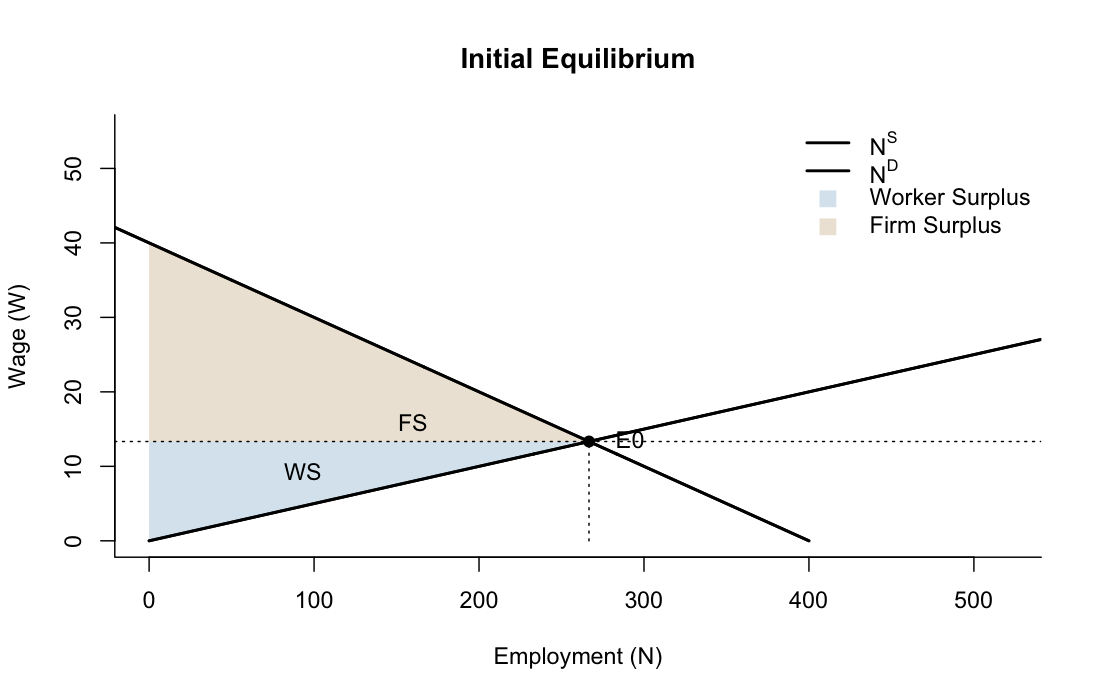
\includegraphics[width=0.91\linewidth]{1aaa}.


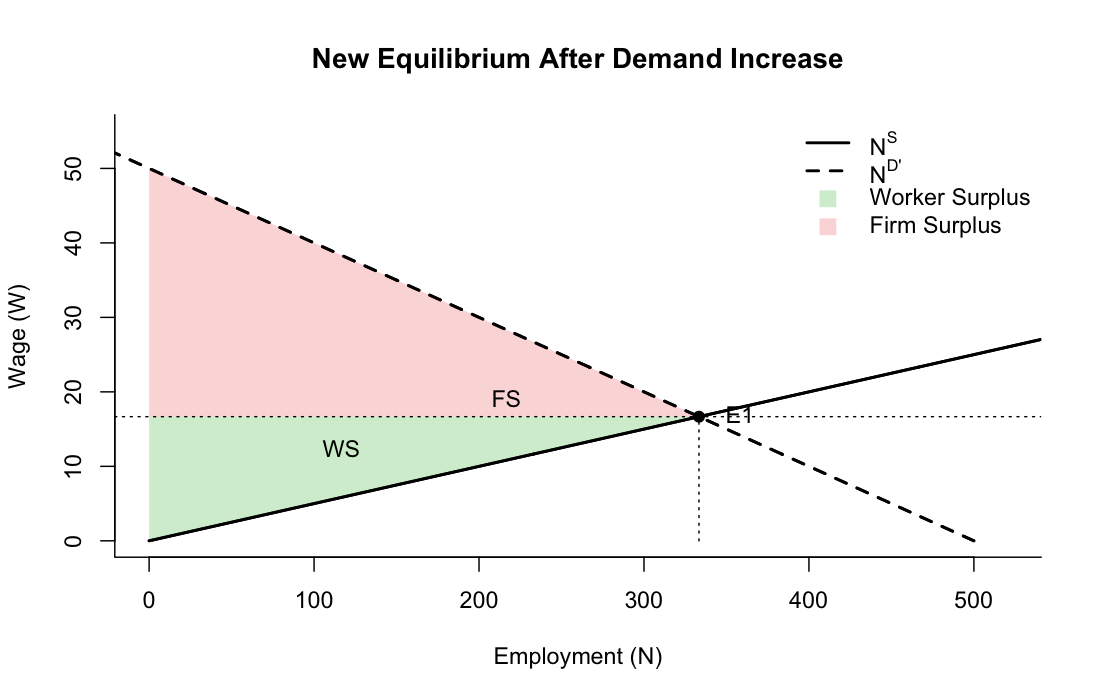
\includegraphics[width=0.91\linewidth]{1bb}.

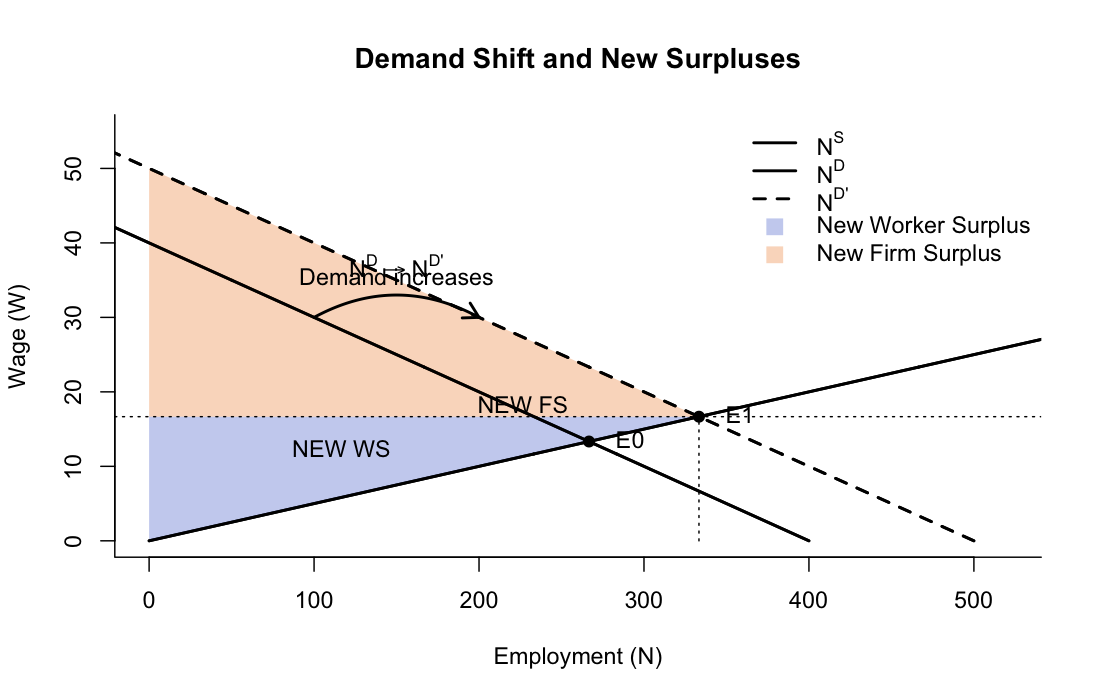
\includegraphics[width=0.91\linewidth]{1c}.

\subsection*{(d) Demand increases to $N^D=500-10W$}
New equilibrium:
\[
20W = 500 - 10W \Rightarrow 30W=500 \Rightarrow W_1=\frac{50}{3}\approx 16.67,
\]
\[
N_1 = 20W_1 = 20\cdot \frac{50}{3}=\frac{1000}{3}\approx 333.33.
\]
\textbf{Explanation:} Higher labour demand bids up wages; higher wages induce greater labour supply, so both $W$ and $N$ rise.



\section*{2. Payroll Tax Incidence (employer payroll tax $T=5$)}

Use original market from Problem 1. Let $W$ be the \emph{wage received by workers}. With an employer tax $T$, the firm pays $W+T$.

\subsection*{(a) New demand in terms of workers' wage}
Original demand is $N^D=400-10(\text{firm cost})$. Firm cost is $W+T$, so:
\[
N^D_{\text{tax}}(W)=400-10(W+T).
\]
With $T=5$:
\[
N^D_{\text{tax}}(W)=400-10W-50=350-10W.
\]

\subsection*{(b) New wages: workers vs firms}
Equilibrium with tax:
\[
20W = 350 - 10W \Rightarrow 30W=350 \Rightarrow W_{\text{worker}}=\frac{35}{3}\approx 11.67.
\]
Firm's cost per worker:
\[
W_{\text{firm}}=W_{\text{worker}}+T=\frac{35}{3}+5=\frac{50}{3}\approx 16.67.
\]

\subsection*{(c) New employment}
\[
N_{\text{tax}}=20W_{\text{worker}}=20\cdot\frac{35}{3}=\frac{700}{3}\approx 233.33.
\]

\subsection*{(d) Tax burden (per worker)}
Pre-tax wage from Problem 1 is $W^*=\frac{40}{3}$.

Worker burden:
\[
W^* - W_{\text{worker}} = \frac{40}{3}-\frac{35}{3}=\frac{5}{3}\approx 1.67.
\]
Firm burden:
\[
W_{\text{firm}}-W^*=\frac{50}{3}-\frac{40}{3}=\frac{10}{3}\approx 3.33.
\]
Check: $\frac{5}{3}+\frac{10}{3}=5=T$.

\subsection*{(e) Deadweight loss (triangle)}
Employment falls by:
\[
\Delta N = N^* - N_{\text{tax}}=\frac{800}{3}-\frac{700}{3}=\frac{100}{3}.
\]
The wedge per worker is $T=5$. DWL is the triangle:
\[
DWL = \frac12 \cdot T \cdot \Delta N
= \frac12\cdot 5 \cdot \frac{100}{3}
= \frac{250}{3}\approx 83.33.
\]

\figplaceholder{Problem 2: Payroll tax incidence}{Show demand shifting down; show wedge $T$ between firms' and workers' wages at the new equilibrium.}


\vspace{0.8em}

\section*{3. Labour Demand: Competitive vs Monopolist Output Market}

\subsection*{Competitive firm}
Given:
\[
MPP_N=50-2N,\qquad P=10.
\]
\textbf{(a) Labour demand.} Value of marginal product:
\[
VMP_N = P\cdot MPP_N = 10(50-2N)=500-20N.
\]
Hiring rule: hire until $VMP_N=W$:
\[
W = 500 - 20N \quad \Rightarrow \quad N(W)=\frac{500-W}{20}.
\]

\textbf{(b) If $W=200$, employment:}
\[
200=500-20N \Rightarrow 20N=300 \Rightarrow N_C=15.
\]

\subsection*{Monopolist}
Given:
\[
P=20-Q,\qquad Q=10N.
\]
\textbf{(c) Marginal revenue without calculus (discrete change).}
Total revenue:
\[
TR(Q)=P\cdot Q=(20-Q)Q=20Q-Q^2.
\]
Define marginal revenue as the additional revenue from selling one more unit:
\[
MR(Q)\equiv TR(Q+1)-TR(Q).
\]
Compute:
\[
TR(Q+1)=20(Q+1)-(Q+1)^2=20Q+20-(Q^2+2Q+1)=20Q+19-Q^2-2Q,
\]
\[
TR(Q)=20Q-Q^2.
\]
So:
\[
MR(Q)=TR(Q+1)-TR(Q)=\big(20Q+19-Q^2-2Q\big)-\big(20Q-Q^2\big)=19-2Q.
\]
(This is the discrete analogue of the familiar linear-demand result.)

\textbf{(d) Marginal revenue product of labour.}
Since $Q=10N$, approximate $MR$ at the firm’s output level using $Q=10N$:
\[
MR(N)=19-2(10N)=19-20N.
\]
Each extra worker adds 10 units of output ($Q=10N$), so:
\[
MRP_N \approx MR(N)\cdot 10 = 10(19-20N)=190-200N.
\]
Hiring rule under monopoly: $MRP_N=W$.

\textbf{(e) Compare employment at $W=200$.}
Monopoly:
\[
190-200N = 200 \Rightarrow -200N=10 \Rightarrow N_M=-0.05.
\]
Negative employment is impossible, so the firm chooses:
\[
N_M=0.
\]
Competition gave $N_C=15$.

\textbf{Interpretation:} Monopoly reduces labour demand because marginal revenue is below price once output is positive, lowering the marginal benefit of hiring labour.

\figplaceholder{Problem 3: Competitive vs monopoly labour demand}{Plot $VMP_N$ and $MRP_N$; show that at a given $W$, monopoly hires less (here $N_M=0$).}

\hrule
\vspace{0.8em}

\section*{4. Basic Monopsony Model (no calculus)}

Supply to the firm:
\[
W(N)=10+0.5N,
\quad\text{and}\quad
VMP_N=100-N.
\]

\subsection*{(a) Total labour cost}
\[
TLC(N)=W(N)\cdot N=(10+0.5N)N=10N+0.5N^2.
\]

\subsection*{(b) Marginal cost of labour (discrete additional cost)}
Define:
\[
MC(N)\equiv TLC(N+1)-TLC(N).
\]
Compute:
\[
TLC(N+1)=10(N+1)+0.5(N+1)^2=10N+10+0.5(N^2+2N+1),
\]
\[
TLC(N)=10N+0.5N^2.
\]
So:
\[
MC(N)=\Big(10N+10+0.5N^2+N+0.5\Big)-\Big(10N+0.5N^2\Big)=N+10.5.
\]

\subsection*{(c) Profit-maximizing employment and wage}
Monopsony hires where $MC$ equals marginal benefit ($VMP_N$):
\[
N+10.5 = 100 - N \Rightarrow 2N=89.5 \Rightarrow N_M=44.75.
\]
Wage paid comes from supply:
\[
W_M=10+0.5(44.75)=10+22.375=32.375.
\]
(If you restrict $N$ to integers, the closest are $N=45$ with $W=32.5$; both are acceptable depending on conventions.)

\subsection*{(d) Competitive benchmark}
Competitive equilibrium solves $W(N)=VMP_N$:
\[
10+0.5N = 100 - N \Rightarrow 1.5N=90 \Rightarrow N_C=60,
\quad W_C=10+0.5(60)=40.
\]

\subsection*{(e) Monopsony wage gap}
Using the continuous solution:
\[
W_C-W_M = 40 - 32.375 = 7.625.
\]
(With integer approximation $N=45$, the gap is $40-32.5=7.5$.)

\figplaceholder{Problem 4: Monopsony}{Plot supply $S$, marginal cost $MC$ (above $S$), and demand $VMP_N$. Mark $(N_M,W_M)$ and $(N_C,W_C)$.}

\hrule
\vspace{0.8em}

\section*{5. Minimum Wage under Monopsony ($\bar W=50$)}

From Problem 4:
\[
W(N)=10+0.5N,\qquad VMP_N=100-N.
\]
A minimum wage $\bar W=50$ means the firm can hire workers at wage 50 up to the amount supplied at 50.

\subsection*{(a) Will employment increase or decrease?}
Compare $\bar W$ with the competitive wage $W_C=40$.
Since $\bar W=50>W_C$, it is above the competitive level, so employment will be \emph{below} the competitive level.

\subsection*{(b) New marginal cost under the minimum wage}
Find how many workers are willing to work at $50$:
\[
50 = 10+0.5N \Rightarrow 0.5N=40 \Rightarrow N=80.
\]
For $N\le 80$, the firm can hire at constant wage 50, so the additional cost of one more worker is approximately $MC=50$ over that range.

\subsection*{(c) Employment choice}
Hire where marginal benefit equals marginal cost:
\[
VMP_N=\bar W \Rightarrow 100-N=50 \Rightarrow N=50.
\]
This is feasible since $50\le 80$.

\subsection*{(d) Efficiency-enhancing?}
No. Minimum wages can raise employment in monopsony only when set between $W_M$ and $W_C$ (moderate). Here $\bar W>W_C$, so employment is pushed below the efficient/competitive level.

\figplaceholder{Problem 5: Minimum wage in monopsony}{Add a horizontal line at $\bar W=50$. Show the firm chooses where $VMP_N=50$.}

\hrule
\vspace{0.8em}

\section*{6. Perfect Monopsonistic Wage Discrimination (no calculus)}

Perfect discrimination means each worker is paid their reservation wage, so hiring one more worker does not require raising wages for others. The marginal cost of hiring equals the supply schedule.

Thus the firm hires where:
\[
VMP_N = W(N).
\]
So:
\[
100-N = 10+0.5N \Rightarrow 90=1.5N \Rightarrow N_D=60.
\]

\subsection*{(b) Compare employment}
\[
N_M \approx 44.75\ (\text{or }45),\qquad N_D=60,\qquad N_C=60.
\]

\subsection*{(c) Worker surplus under perfect discrimination}
Each worker is paid exactly their reservation wage, so economic rent is zero:
\[
WS=0.
\]

\subsection*{(d) Why efficient employment but different distribution?}
Employment is efficient because the hiring condition matches the competitive efficiency condition $VMP_N=W(N)$. Distribution differs because the firm captures the surplus that would otherwise accrue to workers as rents.

\figplaceholder{Problem 6: Perfect discrimination vs monopsony}{Show that discrimination moves the choice from $MC=VMP$ (monopsony) to $S=VMP$ (competitive employment).}

\hrule
\vspace{0.8em}

\section*{7. Short Run vs Long Run Labour Supply to the Firm (no calculus)}

Short-run supply:
\[
W(N)=20+0.2N,
\]
long-run supply is perfectly elastic at:
\[
W=40,
\]
and demand is:
\[
VMP_N=100-2N.
\]

\subsection*{(a) Short-run equilibrium (use discrete marginal cost)}
Total labour cost:
\[
TLC(N)=W(N)\cdot N=(20+0.2N)N=20N+0.2N^2.
\]
Discrete marginal cost:
\[
MC(N)=TLC(N+1)-TLC(N).
\]
Compute:
\[
MC(N)=0.4N+20.2.
\]
Set $MC=VMP$:
\[
0.4N+20.2 = 100-2N
\Rightarrow 2.4N = 79.8
\Rightarrow N_{SR}=33.25.
\]
Short-run wage from supply:
\[
W_{SR}=20+0.2(33.25)=26.65.
\]

\subsection*{(b) Long-run equilibrium employment}
In long run, the firm takes wage 40 and hires where:
\[
VMP_N=40 \Rightarrow 100-2N=40 \Rightarrow 2N=60 \Rightarrow N_{LR}=30.
\]

\subsection*{(c) Why wage falls in the long run (intuition)}
Short run: recruiting more workers requires raising wages (limited mobility/frictions), so the firm faces an upward-sloping supply and higher marginal hiring cost.
Long run: mobility/entry makes labour supply to the firm highly elastic at the market wage (here 40), so wages are determined in the market rather than by firm-level recruitment.

\subsection*{(d) Graph}
\figplaceholder{Problem 7: Short-run vs long-run supply}{Plot $VMP_N$, short-run supply and $MC$, and long-run horizontal supply at $W=40$. Mark $(N_{SR},W_{SR})$ and $(N_{LR},40)$.}

\end{document}